%%
%% This is file `sample-sigconf.tex',
%% generated with the docstrip utility.
%%
%% The original source files were:
%%
%% samples.dtx  (with options: `sigconf')
%% 
%% IMPORTANT NOTICE:
%% 
%% For the copyright see the source file.
%% 
%% Any modified versions of this file must be renamed
%% with new filenames distinct from sample-sigconf.tex.
%% 
%% For distribution of the original source see the terms
%% for copying and modification in the file samples.dtx.
%% 
%% This generated file may be distributed as long as the
%% original source files, as listed above, are part of the
%% same distribution. (The sources need not necessarily be
%% in the same archive or directory.)
%%
%% The first command in your LaTeX source must be the \documentclass command.
\documentclass[sigconf]{acmart}

% TODO remove XD
\usepackage{xcolor}
\newcommand{\secfunc}[1]{{\color{magenta}#1}}
\newcommand{\mention}[1]{{\color{cyan}#1}}
\newcommand{\plan}[1]{{\color{purple}#1}}
\newcommand{\bp}[1]{{\color{violet}#1}}
\newcommand{\draft}[1]{{\color{blue}#1}}
\newcommand{\review}[1]{{\color{black}#1}}
\newcommand{\todo}[1]{{\color{orange}(#1)}}

\usepackage{listings}
\usepackage{tabularx}
\usepackage{cleveref}

%%
%% \BibTeX command to typeset BibTeX logo in the docs
\AtBeginDocument{%
  \providecommand\BibTeX{{%
    \normalfont B\kern-0.5em{\scshape i\kern-0.25em b}\kern-0.8em\TeX}}}

%% Rights management information.  This information is sent to you
%% when you complete the rights form.  These commands have SAMPLE
%% values in them; it is your responsibility as an author to replace
%% the commands and values with those provided to you when you
%% complete the rights form.
\setcopyright{acmcopyright}
\copyrightyear{2020}
\acmYear{2020}
\acmDOI{10.1145/1122445.1122456}

%% These commands are for a PROCEEDINGS abstract or paper.
\acmConference[Seoul '20]{Seoul '20: Mining Software Repositories Data Showcase}{May 25--26, 2020}{Seoul, South Korea}
\acmBooktitle{Seoul '20: Mining Software Repositories Data Showcase,
  May 25--26, 2020, Seoul, South Korea}
\acmPrice{15.00}
\acmISBN{978-1-4503-9999-9/18/06}


%%
%% Submission ID.
%% Use this when submitting an article to a sponsored event. You'll
%% receive a unique submission ID from the organizers
%% of the event, and this ID should be used as the parameter to this command.
%%\acmSubmissionID{123-A56-BU3}

%%
%% The majority of ACM publications use numbered citations and
%% references.  The command \citestyle{authoryear} switches to the
%% "author year" style.
%%
%% If you are preparing content for an event
%% sponsored by ACM SIGGRAPH, you must use the "author year" style of
%% citations and references.
%% Uncommenting
%% the next command will enable that style.
%%\citestyle{acmauthoryear}

%%
%% end of the preamble, start of the body of the document source.
\begin{document}

%%
%% The "title" command has an optional parameter,
%% allowing the author to define a "short title" to be used in page headers.
\title{LogChunks: A Data Set for Build Log Analysis}

\author{Carolin Brandt}
\author{Annibale Panichella}
\author{Andy Zaidman}
\author{Moritz Beller}

%%
%% By default, the full list of authors will be used in the page
%% headers. Often, this list is too long, and will overlap
%% other information printed in the page headers. This command allows
%% the author to define a more concise list
%% of authors' names for this purpose.
\renewcommand{\shortauthors}{Brandt, et al.}

%%
%% The abstract is a short summary of the work to be presented in the
%% article.
\begin{abstract}
Build logs are the textual by-products that a software build processes
creates, often as part of its Continuous Integration (CI)
pipeline. Build logs are a paramount source of information for
developers when debugging into and understanding a build
failures. Recently, attempts to partly automate this time-consuming,
purely manual activity have come up, such as rule- or
information-retrieval-based techniques.

While still in their infancy, we believe that having a common dataset
to be able to fairly compare different build log analysis techniques
will advance the research area and ultimately increase our
understanding of CI build failures. In this paper, we present
\emph{LogChunks}, a collection of 797 fully annotated Travis CI build
logs from 80 GitHub repositories in 29 programming languages. For each
build log, LogChunks contains a manually labeled log part (chunk)
describing why the build failed. We externally validated the data set
with the developer who caused the original build failure.

The width and depth of the \emph{LogChunks} data set are intended to
make it the default benchmark for automated build log analysis
techniques.
\end{abstract}

%%
%% The code below is generated by the tool at http://dl.acm.org/ccs.cfm.
%% Please copy and paste the code instead of the example below.
%%
%\begin{CCSXML}
%<ccs2012>
% <concept>
%  <concept_id>10010520.10010553.10010562</concept_id>
%  <concept_desc>Computer systems organization~Embedded systems</concept_desc>
%  <concept_significance>500</concept_significance>
% </concept>
% <concept>
%  <concept_id>10010520.10010575.10010755</concept_id>
%  <concept_desc>Computer systems organization~Redundancy</concept_desc>
%  <concept_significance>300</concept_significance>
% </concept>
% <concept>
%  <concept_id>10010520.10010553.10010554</concept_id>
%  <concept_desc>Computer systems organization~Robotics</concept_desc>
%  <concept_significance>100</concept_significance>
% </concept>
% <concept>
%  <concept_id>10003033.10003083.10003095</concept_id>
%  <concept_desc>Networks~Network reliability</concept_desc>
%  <concept_significance>100</concept_significance>
% </concept>
%</ccs2012>
%\end{CCSXML}
%
%\ccsdesc[500]{Computer systems organization~Embedded systems}
%\ccsdesc[300]{Computer systems organization~Redundancy}
%\ccsdesc{Computer systems organization~Robotics}
%\ccsdesc[100]{Networks~Network reliability}

%%
%% Keywords. The author(s) should pick words that accurately describe
%% the work being presented. Separate the keywords with commas.
\keywords{CI, Build Log Analysis, Build Failure, Chunk Retrieval}

%%
%% This command processes the author and affiliation and title
%% information and builds the first part of the formatted document.
\maketitle

\section{Introduction}
Continuous Integration (CI) has become a common practice in software
engineering~\cite{hilton2016usage}.  Many software projects use
CI~\cite{hilton2016usage,staahl2014modeling,beller2017oops} to detect
bugs early~\cite{vasilescu2015quality,duvall2007continuous}, improve
developer productivity~\cite{miller2008hundred,hilton2016usage} and
communication~\cite{downs2012ambient}.  CI builds produce logs which
report the results of the steps within the build.  These build logs
contain a lot of valuable information for developers and researchers,
for example: descriptions of compile errors, linter warnings or failed
tests~\cite{beller2017oops,seo2014programmers,vassallo2017a-tale}.

However, build logs can be verbose and large---sometimes in excess of
50 MB of ASCII text ~\cite{beller2017oops}---making them inadequate
for direct human consumption. Therefore, to support developers and
researchers in efficiently making use of the information within build
logs, we must at least semi-automatically retrieve the chunks of the
log that describe the targeted information.

There are different techniques to retrieve information chunks from CI
build logs. Beller et al. use a rule-based system of regular
expressions to analyze logs from Travis CI~\cite{beller2017oops}.
Such regular expressions are developed by looking at exemplary build
logs.  Vassallo et al.\ wrote a custom parser to gather information
for build repair hints~\cite{vassallo2018un-break}.  Recently, Amar et
al.\ reduced the number of lines for a developer to inspect by
creating a diff between logs from failed and successful
builds~\cite{amar2019mining}.

These approaches have various strengths and weaknesses: Regular
expressions are exact, but tedious and error-prone to
maintain~\cite{michael2019regexes}.  Custom parsers are powerful
though fragile in light of changes in the log structure. Diffing
between failed and successful logs can reduce the information to be
processed, but is at best semi-automatic~\cite{amar2019mining}.

At the moment there is only anecdotal evidence on the performance of
these techniques and when a technique should be preferred over its
alternatives.  In fact, there is no data set available to support the
creation of such a benchmark of build log analysis techniques.
Following Sim et al., a benchmark gives us the chance to ``increase
the scientific maturity of the area''~\cite{sim2003using} of build log
analysis by evaluating and comparing research contributions.

Thus, in this paper, we present \emph{LogChunks},\footnote{LogChunks
  is openly available on Zenodo: \todo{insert zenodo link}} a
collection of 797 Travis CI build logs from 80 GitHub repositories in
29 programming languages.  For each build log, we manually labeled
the chunk describing why the build failed.  The data set also provides
keywords the authors would use to search for the labeled log chunk and
categorizes the log chunks according to their format within the log.

\todo{mention most popular repositories very briefly somewhere?}
\todo{Match subsection titles with descriptions in picture}
\todo{80x -> 80}
\begin{figure}[tbp]
	\centering
	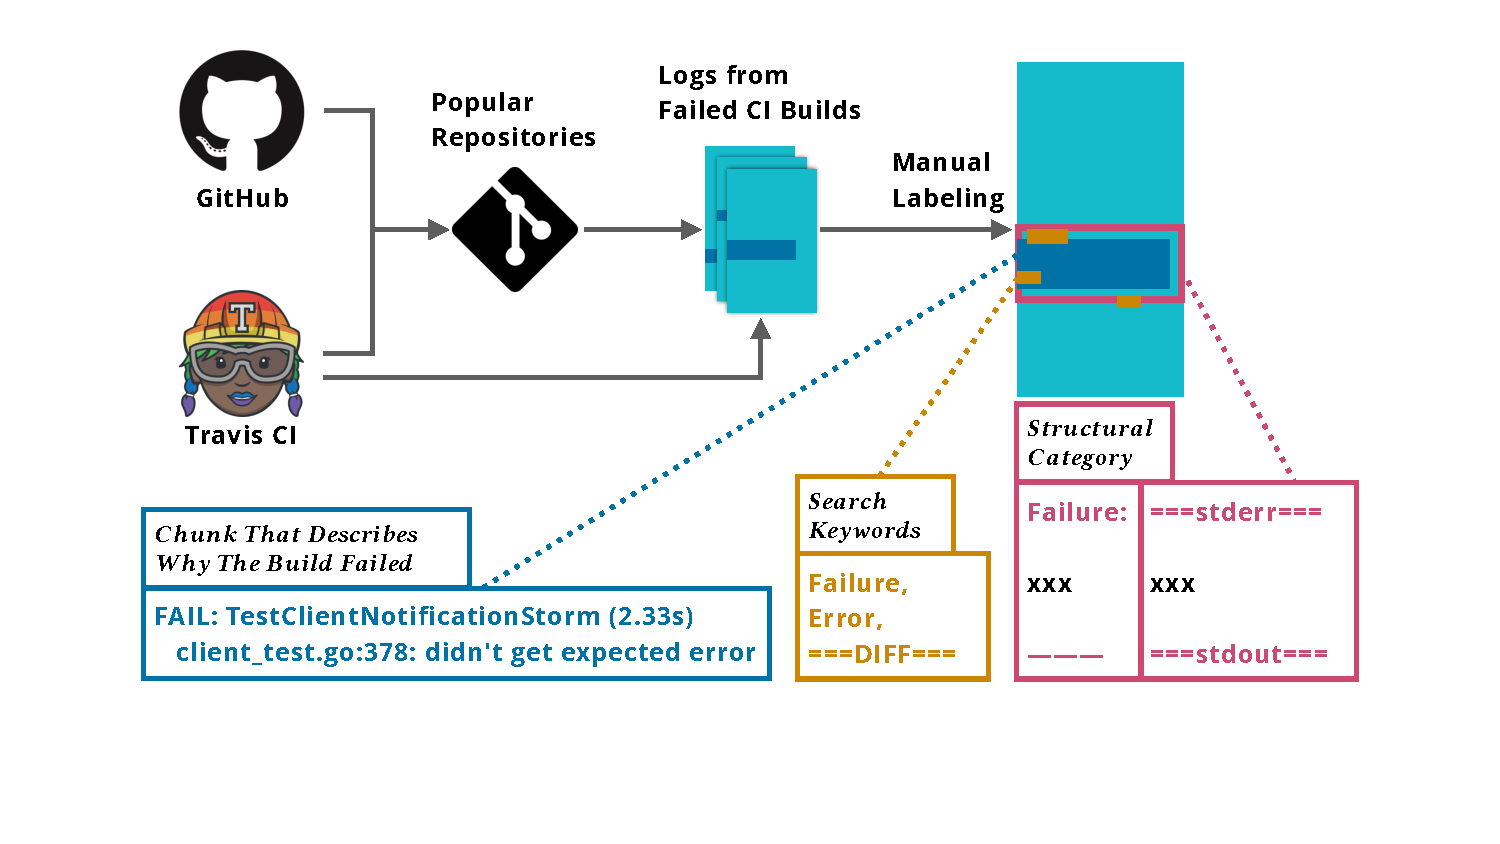
\includegraphics[width=\columnwidth, trim={2cm 2cm 2cm 0.5cm}, clip]{overview.pdf}
	\caption{Overview of \emph{LogChunks}}
	\label{fig:lc-overview}
\end{figure}

\section{Creating LogChunks}
This section presents how we gathered the logs and our manual labeling process.
\label{sec:data-collection}

\subsection{Log Collection}
In this section, we describe how we created \emph{LogChunks} along the
overview in \Cref{fig:lc-overview}. All steps are automatized as Ruby
scripts\todo{link to repo?} and highly configurable.

\paragraph{Repository Sampling}
We first query \emph{GHTorrent}~\cite{gousios2013ghtorrent} for the
most popular languages on GitHub, and subsequently, the most popular
(by number of watchers) repositories for a given language. We measure
popularity by the number of watchers.  We only select repositories
which use Travis CI\@.

For \emph{LogChunks}, we queried GHTorrent on 2018-04-01 for the three
most popular repositories of each of the 30 most popular languages.
Among the resulting repositories are, for example, \texttt{git/git},
\texttt{Microsoft/TypeScript} and \texttt{jwilm/alacritty}.

\todo{we need some reasoning for most popular, our proxy for
  popularity (watchers) -- as is often done, reference --, and ideally, how much
  data we are including}

\paragraph{Build Sampling}
We use a sampling approach using the build status as our stratum.
\todo{What are our strata?}
%We encountered the following statuses during our data collection: created, started, cancelled, passed, errored and failed.

To sample the builds for \emph{LogChunks} we check up to 1,000 builds per repository and keep ten of the status \emph{failed}~\cite{travis2009buildstatus}.
%A Travis CI build is marked as \emph{failed} when it faults in the \texttt{script} section of the build configuration defined by the user.

\paragraph{Log Sampling}
Travis CI builds comprise a number of jobs that actualize a build
process in different environments. Hence, the outcome from different
jobs might be different. For each build in LogChunks, we download the
first job which has the same state as the overall build.

\todo{what does it mean to only have one failed build? wouldn't you
  exclude the entire repository then?}  We inspected the collected
build logs and discarded logs from three repositories.  One had only
one failed build, two others had empty build logs on Travis CI\@.  In
total, we collected 797 logs from 80 repositories spanning 29
languages.

\subsection{Labeling Process}
\label{sec:labeling-process}
After collecting build logs, the first author manually labeled which
text chunk describes why the build failed.  Following that, she
assigned search keywords and structural categories to each log chunk.

\paragraph{Chunk That Describes Why The Build Failed}
For each repository, the labeler skimmed through the build logs and copied out the first occurrence of a description why the build failed.
%They copied out the first continuous description as the \texttt{Chunk}.
They preserved whitespace and special characters, as they might be crucial to detect the targeted substring.
To support learning of regular expressions identifying the labeled substrings the labeler aimed to start and end the labeled substring at consistent locations around the fault description.

\paragraph{Keywords}
We presented the \texttt{Chunk} and ten lines above and below to the labeler.
Their task was to note down three strings they would put into a search field to find this failure description.
The strings should appear in or around the \texttt{Chunk} and is case-sensitive.
There are no limitations on the search string, especially spaces are allowed.

\paragraph{Category}
To label the \emph{structural categories} we presented the \texttt{Chunk} and the surrounding context to the labeler for all logs from a repository.
We asked them to assign numerical categories according to whether the \texttt{Chunk} had the same structural representation.
%The labeler should start the categories with 0 and increase as new ones appear.
%For reproducibility, we presented the logs in chronological build order.


\subsection{Validation}
\label{sec:validation}
\todo{how is the validation embedded in the data set? is there a special flag for validated entries?}

We validated our collected data points in an iterative fashion. First,
we performed an initial inter-rater reliability study with a
co-author, which informed the design of a cross-validation study in
which we contacted over 200 developers.  Our main learning from the
initial internal study was that it is important and difficult to
adequately communicate all decisions and assumptions on how data is
labeled. 

%For \emph{LogChunks} we analyzed around 800 build logs from different repositories and tried to extract the part of the log which describes why the respective build failed.
%As we are not involved in the development of any of the projects within our data set we could only rely on our previous experience with various build logs and systems.
%We only took the logs into account and did not check the related configurations, so it is well possible that we extracted parts that do describe errors but the respective step failing is ignored by the configuration and the build failed for another reason.
%
%The person who probably knows best why a build failed is the one committing the changes which triggered the build.
%If the build was e.g.\ part of a pull request then developer likely inspected the failed build and tried to fix the build so the pull request can be accepted.

In our second validation, we sent out emails to the original
developers whose commits triggered the builds represented in
\emph{LogChunks} and asked them whether the log chunk we labeled
actually describes why the build failed.  This section describes our
survey and discusses our results.

\paragraph{Method}
Using the Travis API, we collected the commit information for each build represented in \emph{LogChunks}.
We grouped all commits triggered by one developer and sent out an email to them.%, asking whether the log part selected during our labeling was indeed describing the reason the build failed.
%Figure~\ref{fig:dev-mail} shows one of the mails sent out.
It included links to the corresponding commits, build overviewm and log file.
We asked the developers to fill out a short form in case our extraction was not correct.
%Look at Figure~\ref{fig:dev-survey} to get an impression of the survey.
In the survey, we asked the developer to paste in the log part actually describing the failure reason or describe in their own words why our original extraction was incorrect.

\paragraph{Results}
In total we sent out mails to 246 developers. 32 of these mails could
not be delivered. We received answers from 61 developers, corresponding to
144 build logs (response rate: 24.8\%).

Of the 144 answers, 132 indicated our extraction was correct.
%26 answered either ``close, but not quite correct'' or ``no, the build failed for another reason''.
We manually inspected the 26 negative answers and found that some stated that the proposed extraction did not show the whole description of why the build failed.
This is because we had to trim long chunks to keep the mails readable.

After adjusting for these answers, 12 answers remained that stated that our labeled log chunk was not correct.

\paragraph{Discussion}
We believe that our developer survey highly strengthens the trust in
the validity of the labeled log chunks.  The study received answers
for about 18\% of the data in \emph{LogChunks}.  After manual
correction, 91\% of the received answers indicated our labeled chunks
were accurate.  One possible threat regarding the high number of
correct answers is that, since we show the error message we extracted,
it might be operationally easier for developers to validate it, rather
than search for it in a long log file. To alleviate this problem, we
made it as easy to confirm as to reject an extracted log chunk. We
only ask for more details (the correct log chunk) in a second step.

One of our 12 incorrect extractions only showed a warning and the
developer proposed to also include the line stating that warnings are
treated as errors. In others, we labeled the error message of an error
that was later ignored.


\section{Data Schema}
\label{sec:data-schema}

This section presents the internal structure and data schema of
\emph{LogChunks}. In principle, LogChunks comprises automatically
retrieved and manually cross-validated data.

%We give a description of the manually labeled data.
%\emph{LogChunks} has two top level folders, \texttt{build-failure-reason} and \texttt{logs}.
%Each contains folders representing the main languages of the repositories in \emph{LogChunks}.
LogChunks comprises information on \todo{x} build logs, which are organized in folders for each language and repository.
Within a repository folder, there are folders for each of the general build status ('successful', 'failed', ...), which contain the entire unaltered log files.
% the logs are separated according to build status.
%Currently, \emph{LogChunks} only contains logs from \texttt{failed} builds.
%The build status folder contains the full logs in files named with the ID of the build that produced the log.
For each repository, \emph{LogChunks} gives about 10 \texttt{Examples}.
\Cref{tab:data-in-example} presents the data LogChunks contaians for an examplatory build from koalaman@shellcheck each example.

The top-level folder \texttt{build-failure-reason} contains the manually labeled data of \emph{LogChunks}.
The data set contains an XML file for each repository: \texttt{\textless repository\_owner\textgreater @\textless repository\_name\textgreater.xml}.
Listing~\ref{lst:examples} presents the schema of these XML files.

Following, this section defines in more detail the labeled log chunk, search keywords and structural categories.

\lstset{
  language=XML,
  morekeywords={Examples, Example, Log, Keywords, Category, Chunk},
  postbreak=\mbox{\textcolor{cyan}{$\hookrightarrow$}\space},
	frame=single,
	escapeinside=**
}
\begin{figure}[]
	\centering
\begin{lstlisting}[breaklines=true]
<Examples>
  <Example>
    <Log>C/php@php-src/failed/529279089.log</Log>
      <Keywords>ERROR, FAIL, DIFF</Keywords>
      <Category>0</Category>
      <Chunk>001+ ** ERROR: process timed out **
001- OK.
========DONE========
FAIL Bug #60120 (proc_open hangs)</Chunk>
  </Example>
  ...
</Examples>
\end{lstlisting}
	\caption{Example XML file from \emph{LogChunks} \todo{Isn't this exactly the same as Figure 2? Only keep one?}}
	\label{lst:examples}
\end{figure}


\begin{figure*}[htbp]
\centering
\begin{tabularx}{\textwidth}{@{}lXlX@{}}
  \toprule
  Data & Description & Unit & Example \\
  \midrule
  Log & Relative path to the input build log & Path & \tt{Haskell/koalaman@shellcheck\newline/failed/501296412.log} \\
  Chunk & Log chunk that describes why the build failed & String & \tt{shellcheck.hs:442:19: error:
    Variable not in scope: doesPathExist :: [Char] -> IO Bool} \todo{is this strictly one?} \\ 
  Keywords & Keywords the authors would use to search \todo{only search or also actually FIND it?} for the log chunk & List of Strings & \tt{Failures, FAILURE, FAILED} \\ 
  Category & Categorization of the structural representation of the log chunk within the build log \todo{can you explain what this means?} & Integer & \tt{0}\\
  \todo{what about validation info?}\\
  \bottomrule
\end{tabularx}
\caption{Examplary, complete data excerpt from \emph{LogChunks} for a failed build in \tt{koalaman@shellcheck}.}
\label{tab:data-in-example}
\end{figure*}

\todo{Including Figure 3 as a running example}
\paragraph{Chunk That Describes Why The Build Failed}
The \texttt{Chunk} is the substring of the build log that describes why the build failed.
This can, for example, be the failing test case or a compiler error.
In cases where the reason \emph{why} the build failed is contained in a log file external to the main build log, the \texttt{Chunk} includes only the fact \emph{that} the build failed.\todo{what does this look like?} In \Cref{tab:data-in-example}, this is a compile error where a variable did not exist in the current scope.

%Wherever possible, it does \emph{not} include the log statements describing \emph{that} the build failed, but the description of \emph{why} it failed.
%For a few logs we were unable to define the section detailing why the build failed, e.g.\ because this information was logged in another log file.
%In these instances the \texttt{Chunk} contains the lines describing that the build failed.

\paragraph{Keywords}
The \texttt{Keywords} contain a list of one to three \todo{find different word to explain it with} keywords appearing within the \texttt{Chunk} or in the area around it in the build log.
We selected keywords the authors would use to search for the log \texttt{Chunk} after analyzing about 800 build logs manually.\todo{This needs more explanation! Why these keywords (as opposed to others?)}
Some keywords from \emph{LogChunks} are: ``\texttt{FAIL}'', ``\texttt{Error}'', ``\texttt{=DIFF=}'' or ``\texttt{ERR!}''.

\paragraph{Category}
For each repository, we assign \emph{structural categories} to the chunks.
The structural category compares how \texttt{Chunk}s are represented within the build log.
Build tools highlight their error messages with markings, e.g.\ starting each line with ``\texttt{ERROR}'' or surrounding special characters.
Two chunks fall into the same structural categories if they are surrounded by the same markings.
Listing \ref{lst:same-category} presents a log chunk from the same category as the log chunk from Listing \ref{lst:examples}.
In comparison to that, Listing \ref{lst:different-category} presents a log chunk which is formatted differently within the log file.
%For most cases, two \texttt{Chunk} examples that fall into one category are outputted either within the same build phase or by the same build tool.
For each repository, the structural categories are represented as integers, starting at 0 and increased with the next appearing category in chronological build order.

\begin{figure}[tbp]
	\centering
\begin{lstlisting}[breaklines=true]
========DIFF========
*{\color{cyan}-=-=-=-=-=-}*
005+     Parameter #1 [<optional> $flags]
005-     Parameter #1 [<optional> $ar_flags]
========DONE========
FAIL Bug#71412 ArrayIterator reflection 
*{\color{cyan}-=-=-=-=-=-}*
TEST 9895/13942 [2/2 test workers running]
\end{lstlisting}
	\caption{Log chunk from the \emph{same} structural category as the log chunk presented in Listing \ref{lst:examples}, ``{\color{cyan}-=-=-=-=-=-}'' separates the log chunk from the context}
	\label{lst:same-category}
\end{figure}

\begin{figure}[tbp]
	\centering
\begin{lstlisting}[breaklines=true]
[0K$ ./sapi/cli/php run-tests.php -P ...
*{\color{cyan}-=-=-=-=-=-}*
Illegal switch 'j' specified!
*{\color{cyan}-=-=-=-=-=-}*
Synopsis:
\end{lstlisting}
	\caption{Log chunk from a \emph{different} structural category than the log chunk presented in Listing \ref{lst:examples}}
  %, ``{\color{cyan}-=-=-=-=-=-}'' separates the log chunk from the context}
	\label{lst:different-category}
\end{figure}


%\section{Applications}
%This section possible use cases for \emph{LogChunks} and outlines how we previously applied it to compare different build log analysis techniques.
\section{Potential Use Cases}

%\subsection{Potential Use Cases}
\emph{LogChunks} can be the basis for a range of further studies:

\paragraph{Benchmarking Build Log Analysis Techniques}
LogChunks is a spin-off from research in which we compared three different log chunk retrieval techniques protypically. %\todo{cite journal paper (or preprint?)}.
\emph{LogChunks} can be a benchmark to evaluate other build log analysis techniques.
For example, we can use the data set to investigate how reliably the diff-based approach of Amar et al.~\cite{amar2019mining} retrieves a build failure reason.

\paragraph{Support Build Log Classification Algorithms}
Various researchers are examining why CI builds fail and use build logs as a data source~\cite{seo2014programmers,vassallo2017a-tale}.
They write custom parsers and classifiers to categorize builds according to why a build failed.
The manually labeled chunk can help researchers locate the source for their classification algorithms and cross-validate their data.

\paragraph{Analysis of Keywords Used to Search for Build Failure Descriptions}
\emph{LogChunks} provides keywords that the authors would use to search for the chunk describing why the build failed.
Analyzing these can help us understand how users process build logs and which keywords a tool should use to mark an error description.
We can also recommend users which search keywords they should use to find why the build failed.
\todo{Isn't this pretty simple and not really worth a research paper? If it is too trivial, we should probably not mention it here.}

\paragraph{Studying Conversations about Build Failures}
Researchers are looking into conversations of developers surrounding CI builds and pull requests \todo{citation pending}
%TODO Caro: nathan cassee (with Alexander Sebrenik) did this in his master thesis (paper got accepted, will get link when preprint is finished), did not find others yet that do this}.
The chunks describing why a build failed, or the results of build log analysis techniques trained on them, can support these researchers to detect when a conversation participant is referring to the build failure described in the log.
\todo{Similar comment: This is a bit too narrow. But perhaps we can merge the two in one and say researchers doing research around the topic of build logs, such as ... user studies on keyword retrievala and conversations?}

\todo{ Andy also proposed: automatic creation of issue reports on GitHub with extracted info: sounds okay, but build failures are to be fixed faster than a GH issue I would say}
\todo{I think this proposal is again too narrow: but what about further automatic on-ward processing? Even if small, perhaps reinforcement learning might be feasible ...}

% \subsection{Chunk Retrieval Evaluation}
% We created \emph{LogChunks} to evaluate and compare different chunk retrieval techniques for build logs.
% The first technique is based on synthesizing programs from examples using the Microsoft PROSE library.
% A user provides a small number of examples to describe which text part the program should extract.
% PROSE then synthesizes a program of regular expressions that is consistent with these examples.
% We compared this extraction technique to a text similarity approach, which selects the lines of a build log which are most similar to the ones in the given user examples.
% Lastly, we investigated searching for keywords that are associated with the given user examples.

% The log chunks in this data set provided the examples for these techniques, the keywords were used to configure the keyword search.
% The structural categories enabled us to measure how structurally similar the examples have to be for a technique to be applicable.

% Our results show that program synthesis is well suited to retrieve information chunks from build logs when the targeted information is always presented in a structurally identical way and the user requires a high confidence in the precision and recall of the output.
% Using text similarity is advisable when precision is valued higher than recall and we recommend keyword search when recall is valued higher than precision.
% We present more detailed results, background and our study design in \todo{ref (preprint or so?) of full journal paper (or thesis?)}.

\section{Related Data Sets}
\label{sec:related-data-sets}
This section presents existing data sets of CI build logs and how
\emph{LogChunks} differs from them.

\subsection{TravisTorrent}
\emph{TravisTorrent}~\cite{beller2017travistorrent} collects a broad
range of metadata about Travis CI builds\@.  It combines data
accessible through the public Travis CI and GitHub APIs and through
GHTorrent~\cite{gousios2013ghtorrent}. Similar to LogChunks, among the
metadata are the failing test cases. However, TravisTorrent obtained
these through a manually developed parser, which only supports
specific Ruby test runners and Java Maven or JUnit logs. Anecdotally,
many of the failing tests are at least incomplete and lack
validation. By contrast, \emph{LogChunks} provides manually labeled
and two-fold cross-validated data of why builds failed, not only for
failing tests like TravisTorrent, but for all possible build-failing
errors.


\subsection{Travis CI Build Log Data Set}
\todo{I would remove this as it is not really related because it does not contain labels?}
Loriot et al.~\cite{loriot2019dataset, loriot2019styler} collected Travis CI build logs from 130 GitHub repositories to analyze their use of the Checkstyle plugin.
They selected Maven repositories that included the Checkstyle plugin.
Their data set only provides the plain build logs, whereas \emph{LogChunks} additionally provides manually labeled data about the chunk describing why a build failed.

\todo{What about the related data set I showed you and Georgios also mentioned? (Forgot exact name but don't have Internet so cannot look it up.)}

\section{Future Extensions to LogChunks}

In this section, we describe LogChunk's current limitations and future improvements and extensions we are planning.

\paragraph{Chunk as One Consecutive Substring}
The manually labeled \texttt{Chunk} contains only one continuous substring of the log text.
The reason a build failed could be described at multiple locations within the log.
We propose to extend \emph{LogChunks} to contain multiple substrings of the log text.

\paragraph{Include More Repositories and Logs}
\emph{LogChunks} encompasses a range of repositories from various main development languages, though only 10 logs from each repository.
%This stems from the high effort necessary for the manual data labeling process.
Including more logs and repositories into \emph{LogChunks} will strengthen it as a benchmark to compare build log analysis techniques.

\paragraph{Classification of the Build Failure Cause}
Our data set contains no further classification according to the cause of the failure.
As researchers are investigating why CI builds fail, a useful extension is to annotate cause of the build failure for each log.
\todo{Example: such as this is due to tests, compilation, ...?}

\paragraph{Other Targeted Information Chunks}
Build log analysis is not limited to retrieving the chunk describing why a build failed.
\emph{LogChunks} can be extended with further information targets such as descriptions of warnings, build infrastructure and more.
\todo{a rich description of all info contained in a build log?}

\paragraph{Validation of Search Keywords}
The keywords \emph{LogChunks} provides are based on the experience of the authors gained from analyzing around 800 build logs.
Next, we propose to evaluate whether these keywords would also be used by developers to find the log chunk describing why a build failed.



\section{Summary}
\label{sec:conclusion}
In this paper, we introduce\emph{LogChunks}, a cross-validated data
set encompassing 797 build logs from 80 projects using Travis CI\@.
For each log, we annotated the log chunk describing why the build
failed and provide keywords a developer would use to search for the
log chunk as well as a categorization of the log chunks according to
their format within the log. \emph{LogChunks} advances the research
field of build log analysis by introducing a benchmark to rigorously
examine research contributions~\cite{sim2003using} and opening various
research possibilites that previously required tedious manual
classification.

%%
%% The acknowledgments section is defined using the "acks" environment
%% (and NOT an unnumbered section). This ensures the proper
%% identification of the section in the article metadata, and the
%% consistent spelling of the heading.

% \begin{acks}
% To Robert, for the bagels and explaining CMYK and color spaces.
% \end{acks}

%%
%% The next two lines define the bibliography style to be used, and
%% the bibliography file.
\bibliographystyle{ACM-Reference-Format}
\bibliography{paper}

%%
%% If your work has an appendix, this is the place to put it.
% \appendix

% \section{Research Methods}

% \subsection{Part One}


\end{document}
\endinput
%%
%% End of file `sample-sigconf.tex'.
